% Credit goes to:
% Adrien Friggeri and Carmine Benedetto whose FancyCV and SmartFancyCV are the basis for my work:
	% https://github.com/neoben/smart-fancy-latex-cv/commits?author=neoben
%!TEX TS-program = XeLaTex / XeLaTex + MakeIndex
%Most of Doug´s data courtesy of https://kingofqueens.fandom.com

\documentclass[a4paper]{friggeri-cv_reccius-experiment}
\usepackage[UTF8,scheme = plain]{ctex}
\usepackage{afterpage}
\usepackage{hyperref}
\usepackage{color}
\usepackage{xcolor}
\PassOptionsToPackage{cmyk}{xcolor}
\usepackage{smartdiagram}
\usepackage{fontspec}
\usepackage{fontawesome}
\usepackage{marvosym}
\usepackage{textcomp}
\usepackage{float} % to position signature
\usepackage{adjustbox}
\usepackage{calc}
\usepackage{enumitem} % to customize indent of bullet points via \itemize
\usepackage{metalogo}
\usepackage{dtklogos}
\usepackage[utf8]{inputenc}	
\usepackage{tikz}
\usetikzlibrary{mindmap,shadows,positioning}
\hypersetup{
    pdftitle={},
    pdfauthor={},
    pdfsubject={},
    pdfkeywords={},
    colorlinks=false,           % no lik border color
    allbordercolors=white       % white border color for all
}
\smartdiagramset{
    bubble center node font = \footnotesize,
    bubble node font = \footnotesize,
    % specifies the minimum size of the bubble center node
    bubble center node size = 0.06cm,
    %  specifies the minimum size of the bubbles
    bubble node size = 0mm,
    % specifies which is the distance among the bubble center node and the other bubbles
    distance center/other bubbles = 0.8cm,
    % sets the distance from the text to the border of the bubble center node
    distance text center bubble = 0.3cm,
    % set center bubble color
    bubble center node color = centergray,
    % define the list of colors usable in the diagram
    set color list = {bubblegray, bubblegray, bubblegray, bubblegray, bubblegray, white, lightgray, lightgray, lightgray, lightgray},
    % sets the opacity at which the bubbles are shown
    bubble fill opacity = 0.7,
    % sets the opacity at which the bubble text is shown
    bubble text opacity = 1,
}

% \addbibresource{bibliography.bib}
\RequirePackage{xcolor}
\definecolor{lightgray}{HTML}{777788}
\definecolor{centergray}{HTML}{B9B9C9}
% you can change ipsgreen to any color you like, but you´ll also have to change it in the reccius-cv-experiment.cls file
\definecolor{ipsgreen}{HTML}{3B6746}

\renewcommand{\baselinestretch}{1.4}

% NAME AND TAGLINE
\begin{document}
\header{陈}{树林}
      {生物信息工程师}
      
\vspace{0.3cm}   
\color{lightgray}\noindent\makebox[\textwidth]{\rule{\paperwidth-0.4cm}{2.5pt}}
% In the aside, each new line forces a line break

%%%%%%%%%%%%%%%%%%%%%%%%%%%%%%%%%%%%%
%%%%%%%%%%%%                 CONTACT                %%%%%%%%%%
%%%%%%%%%%%%%%%%%%%%%%%%%%%%%%%%%%%%%

\begin{info}
    \begin{flushleft}
    
    \small 广州市黄埔区}\hfill{\Large\faMapMarker\thinspace\thinspace\thinspace}\\
    
    \vspace{0.08cm}
    
    {\small 18933973814}\hfill{\LARGE\Mobilefone\thinspace}\\

    \vspace{0.14cm}
    
    \href{mailto:qingyun039@163.com}{{\small\textbf{qingyun039@}163.com}\hfill{\Large\Letter}\hspace{0.6mm}{\small \faMousePointer}}\\

    \href{https://github.com/qingyun039}{{\small qingyun039}\hfill{\LARGE \faGithub\thinspace\thinspace\verythinspace}}\\
    
    \end{flushleft}
\end{info}

%%%%%%%%%%%%%%%%%%%%%%%%%%%%%%%%%%%
%%% %%%%%%%%               SIDE BARS               %%%%%%%%%
%%%%%%%%%%%%%%%%%%%%%%%%%%%%%%%%%%%
\begin{aside}
    ~

% PICTURE
\vspace{-3.5cm}
\begin{figure}[ht]
	\hspace{0.3cm}
	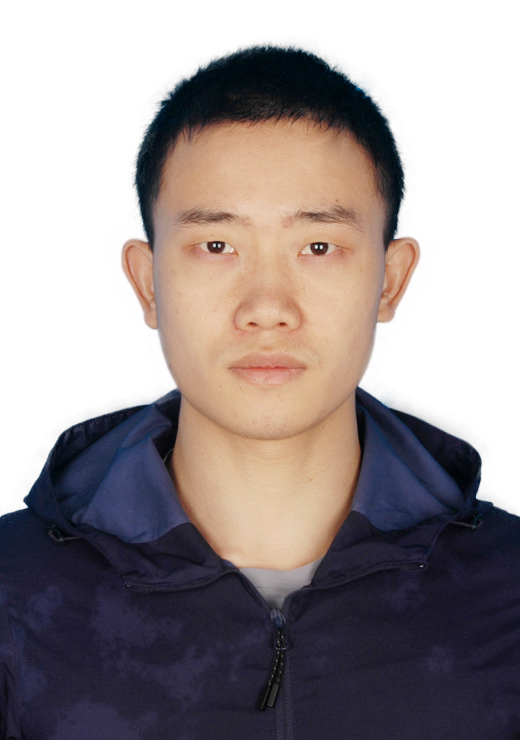
\includegraphics[width=.71\linewidth]{img/Photo1.jpg}
\end{figure}

% SKILLS
\newcommand{\skillspace}{\vspace*{-0.75mm}}
  \vspace{-2.9mm}
  \section{基本信息}\\
  \vspace{3.5mm}
  \begin{tabular}{r@{: }l}
      年龄 & 27岁 \\
      性别 & 男 \\
      籍贯 & 广东韶关 \\
      学历 & 本科 \\
      专业 & 生物信息学 \\
      学校 & 南方医科大学
  \end{tabular}
  \section{生信方向}\\
  \vspace{3.5mm}
    \begin{tikzpicture}[node distance = 7mm, terminal/.style={
    	rectangle, minimum height = 2mm, rounded corners = 1mm, thick, 
    	draw = darkgray, fill = white, align = left}]
    	\node (A) [terminal] {临床检测};
    	\node (B) [terminal, right=2mm of A.east,anchor=west] {遗传(WES/NIPT)};
    	\node (C) [terminal, below=of A.west,anchor=west] {肿瘤伴随诊断};
    	\node (D) [terminal, below=of C.west,anchor=west] {靶向测序};
    	\node (E) [terminal, right=2mm of D.east,anchor=west] {病原微生物(mNGS)};
    	\node (F) [terminal, below=of D.west,anchor=west] {高性能计算集群管理};
    	\node (G) [terminal, below=of F.west,anchor=west] {分析流程搭建}
	\end{tikzpicture}

  \vspace{-2.6mm}
  \section{编程语言}\\
    \vspace{1.7mm}
    \textbf{PERL}\hfill
    
\includegraphics[scale=0.11]{img/IPSGreenDots.png}
    
\includegraphics[scale=0.11]{img/IPSGreenDots.png}
    
\includegraphics[scale=0.11]{img/IPSGreenDots.png}
    
\includegraphics[scale=0.11]{img/IPSGreenDots.png}
    
\includegraphics[scale=0.11]{img/WhiteDots.png}
    
\includegraphics[scale=0.11]{img/WhiteDots.png}\\
    \belowspace
    \textbf{PYTHON}\hfill
    
\includegraphics[scale=0.11]{img/IPSGreenDots.png}
    
\includegraphics[scale=0.11]{img/IPSGreenDots.png}
    
\includegraphics[scale=0.11]{img/IPSGreenDots.png}
    
\includegraphics[scale=0.11]{img/IPSGreenDots.png}
    
\includegraphics[scale=0.11]{img/IPSGreenDots.png}
    
\includegraphics[scale=0.11]{img/WhiteDots.png}\\
    \belowspace
    \textbf{R}\hfill
    
\includegraphics[scale=0.11]{img/IPSGreenDots.png}
    
\includegraphics[scale=0.11]{img/IPSGreenDots.png}
    
\includegraphics[scale=0.11]{img/IPSGreenDots.png}
    
\includegraphics[scale=0.11]{img/WhiteDots.png}
    
\includegraphics[scale=0.11]{img/WhiteDots.png}
    
\includegraphics[scale=0.11]{img/WhiteDots.png}\\
    \belowspace
    \textbf{SQL}\hfill
    
\includegraphics[scale=0.11]{img/IPSGreenDots.png}
    
\includegraphics[scale=0.11]{img/IPSGreenDots.png}
    
\includegraphics[scale=0.11]{img/WhiteDots.png}
    
\includegraphics[scale=0.11]{img/WhiteDots.png}
    
\includegraphics[scale=0.11]{img/WhiteDots.png}
    
\includegraphics[scale=0.11]{img/WhiteDots.png}\\
    \belowspace
    \textbf{RUST}\hfill
    
\includegraphics[scale=0.11]{img/IPSGreenDots.png}
    
\includegraphics[scale=0.11]{img/WhiteDots.png}
    
\includegraphics[scale=0.11]{img/WhiteDots.png}
    
\includegraphics[scale=0.11]{img/WhiteDots.png}
    
\includegraphics[scale=0.11]{img/WhiteDots.png}
    
\includegraphics[scale=0.11]{img/WhiteDots.png}\\~
  
  \vspace{-2.7mm}
  \section{兴趣爱好}\\
  \vspace{3.5mm}
  \begin{itemize}[leftmargin=*, noitemsep]
      \item 跑步、篮球
      \item 读书(红楼梦等古典小说)
      \item 观看电子竞技比赛
  \end{itemize}
  
\end{aside}
~
% LANGUAGES
\newcommand{\belowspace}{\vspace*{0.85mm}}
\begin{textblock*}{\paperwidth}(0cm, 26.15cm)
  \begin{center}
      qingyun039 | 2019-2020\\
      ModernFancyCV template from overleaf
  \end{center}
\end{textblock*}

%%%%%%%%%%%%%%%%%%%%%%%%%%%%%%%%%%%
%%% %%%%%%%%             EDUCATION             %%%%%%%%%%
%%%%%%%%%%%%%%%%%%%%%%%%%%%%%%%%%%%
\newcommand{\eduspace}{\vspace*{0.85mm}}
\newcommand{\eduspaceII}{\vspace*{0.8mm}}
\newcommand{\jobspace}{\vspace*{-4.2mm}}
\vspace{-0.5mm}

\section{项目经验}
\begin{entrylist}

    \entry
    {2022.7\enspace}
    {全外显子组基因检测(WES) | }{\small{达安基因}}
    {\normalsize\textbf{\color{ipsgreen}\faMapMarker\space 广州}}
    {
    负责开发全外显子组基因检测项目的生物信息流程。该项目主要分为两个部分:

    \begin{enumerate}
        \item 流程管理框架
        \item 全外基因检测
    \end{enumerate}

    \hspace{0.4cm}\textbf{流程管理框}架使用数据库记录流程、分析、任务的定义,保存各步骤的完成状态、分析结果,实现多任务并行运行和实时的资源调度
    。使用流程管理框架方便系统开发人员将生物信息流程嵌入到系统中,使用户可以在网页上启动流程、追踪任务状态、查询分析结果。该框架开发后,先后整合全外项目、CNVseq项目、NIPT项目的生信流程。
    
    \hspace{0.4cm}\textbf{全外基因检测}除了包括了基本的SNV/INDEL变异检测外,还包含单个外显子级别的拷贝数变异(CNV)检测、常见动态突变(STR)检测、杂合性缺失/单亲二体(AOH/UPD)检测、线粒体变异检测。其中还有性别校验、亲缘检测、交叉污染检测用于质量控制。该检测流程已与公司的遗传解读系统结合,已可用于实际生产中。\\
    }

    \entry
    {2021.9\enspace}
    {无创产前基因检测(NIPT) | }{\small{达安基因}}
    {\normalsize\textbf{\color{ipsgreen}\faMapMarker\space 广州}}
    {
    负责研发基于MGI平台的无创产前检测(NIPT)生物信息流程,该流程具有以下性能对标结果:

    \begin{itemize}
        \item 稳定检出21、18、13-三体
        \item 正确检出性染色体异常XXX、XO, XYY和XXY还需优化
        \item 可检出大部分拷贝数变异
        \item 较为准确的预测女胎胎儿浓度
    \end{itemize}

    由于其它原因该流程没有用于实际生产中。\\
    }
 
   \entry
    {2019.9\enspace}
    {泛癌基因检测流程 | }{\small{北斗医学检验室}}
    {\normalsize\textbf{\color{ipsgreen}\faMapMarker\space 广州}}
    {
    泛癌基因检测流程覆盖多种类型癌症基因检测,分析结果可用于癌症患者靶向用药、免疫治疗、遗传易感。流程由3人开发完成。本人在流程开发中负责:
    
    \begin{itemize}
        \item 下机数据自动化拆分程序开发
        \item 检测效果评估测试
        \item ctDNA检测流程开发
    \end{itemize}
    
    这套流程已实际应用于生产中,ctDNA流程2020年室间质评成绩90分。\\
    }
    
  \entry
    {2018.5\enspace}
    {健康基因检测报告系统 | }{\small{天一辉远基因科技有限公司}}
    {\normalsize\textbf{\color{ipsgreen}\faMapMarker\space 广州}}
    {健康基因检测报告系统用于出具客户健康基因检测报告。该项目由本人一人开发,使用
    perl作为编写语言,可分为三大模块:基因检测结果及客户信息的输入处理、健康风险分析计算、结果数据渲染及报告生成。该系统实际应用于公司健康业务中,累计生成过1000+份基因检测报告。
    \eduspace\\}

\end{entrylist}
%%%%%%%%%%%%%%%%%%%%%%%%%%%%%%%%%%
%%%%%%%%%%%%       EXPERIENCE       %%%%%%%%%%%%
%%%%%%%%%%%%%%%%%%%%%%%%%%%%%%%%%%
\clearpage
\section{工作经历}
\begin{entrylist}
    \entry
    {2020.12 - 2023.2\enspace}
    {广州达安基因股份有限公司 | }{ \href{https://en.wikipedia.org/wiki/Bioinformatics}{\small 生物信息工程师 \faMousePointer}}
    {\normalsize\textbf{\color{ipsgreen}\faMapMarker\space 广州}}
    {\jobspace
    \begin{itemize}[leftmargin=*, itemsep = 0.1em]
    \item 负责优生优育方向相关项目研发,包括全外、CNVseq、NIPT、无创地贫
    \item 负责肿瘤MSI检测模块开发
    \item 负责平台高性能计算集群(HPC)的管理\\
    \end{itemize}
    }

  \entry
    {2019.7 - 2020.11\enspace}
    {北斗医学检验室 | }{ \href{https://en.wikipedia.org/wiki/Bioinformatics}{\small 生物信息工程师 \faMousePointer}}
    {\normalsize\textbf{\color{ipsgreen}\faMapMarker\space 广州}}
    {\jobspace
    \begin{itemize}[leftmargin=*, itemsep = 0.1em]
    \item 参与生物信息流程开发,测试
    \item 分析肿瘤样本,配合报告人员进行结果解析
    \item 编写生物信息学软件并撰写相关软著
    \item 负责科研项目中一些生信分析工作\\
    \end{itemize}
    }
    
  \entry
    {2018.7 - 2019.5\enspace}
    {天一辉远基因科技有限公司 | }{ \href{https://en.wikipedia.org/wiki/Bioinformatics}{\small 生物信息工程师 \faMousePointer}}
    {\normalsize\textbf{\color{ipsgreen}\faMapMarker\space 广州}}
    {\jobspace
    \begin{itemize}[leftmargin=*, itemsep = 0.1em]
    \item 负责报告系统编写,测试,开发
    \item 参与各类健康基因检测产品的研发,并负责嵌入到报告系统中
    \item 负责报告生成并按照客户要求调整报告\\
    \end{itemize}
    }
    
  \entry
    {2017.7\,-\,2018.5\enspace}
    {精科医学检验所 | }{\href{https://en.wikipedia.org/wiki/Bioinformatics}{\small 生物信息工程师 \faMousePointer}}
    {\normalsize\textbf{\color{ipsgreen}\faMapMarker\space 广州}}
    {\jobspace
    \begin{itemize}[leftmargin=*, noitemsep]
    \item 编写肺癌风险、三高风险,烟酒基因检测报告的生成程序
    \item 尝试构建突变位点网站
    \item 完成上级交代的任务 \\
    \end{itemize}
    }
    
\end{entrylist}

\begin{textblock*}{\paperwidth}(0cm, 26.15cm)
  \begin{center}
      qingyun039 | 2019-2020\\
      ModernFancyCV template from overleaf
  \end{center}
\end{textblock*}

\end{document}